\chapter{Dynamic Programming}

\section*{The Bellman Equation}

In Chapter 10 we studied optimization over time. The constraints (\ref{equa10.1}) expressing increments to stocks or state variables, and the additively separable form (\ref{equa10.3}) of the objective function, were special features that enabled us to express the first-order conditions in a useful special form, namely as the Maximum Principle. Dynamic Programming is an alternative way of solving the same problem. It proves especially useful when time and uncertainty appear together, as they so often do in reality. Let us begin with time to keep the exposition simple, and introduce uncertainty later.

The vectors of initial stocks $y_0$ and terminal stocks $y_{T+1}$ were given when we maximized
\begin{equation*}  \tag{10.3}
\sum\limits_{t=0}^T F(y_t, z_t, t)
\end{equation*}
subject to the constraints 
\begin{equation*}  \tag{10.1}
 y_{t+1} - y_t = Q(y_t, z_t, t)
\end{equation*}
and
\begin{equation*}  \tag{10.2}
  G(y_t, z_t, t) \leq 0
\end{equation*}
for $t=0,1,\dots, T$. Keep the terminal stock requirement fixed for now. As in Chapter 5, we can define the resulting maximum value as a function of the initial stocks, say $V(y_0)$. The vector of derivatives $V_y(y_0)$ will be the vector of the shadow prices of these initial stocks.

The separability of the objective and the constraints allows us to generalize this greatly. Instead of the starting time 0, consider another particular time, say $t = \tau$. For the decisions starting at $\tau$, the only thing that matters about the past is the vector $y_\tau$ of stocks that emerges from the past decisions. We can take that as parametric, and start the whole problem afresh at $\tau$. In other words, we maximize a sum just like (\ref{equa10.3}), but extending only from $\tau$ to $T$, subject to constraints just like (\ref{equa10.1}) and (\ref{equa10.2}), but holding only for $\tau, \tau + 1, \dots T$. Let $V(y_\tau, \tau)$ be the maximum value function of this problem; the explicit argument $\tau$ is necessary because the limit of the summation depends on it. The vector of derivatives $V_y(y_\tau, \tau)$ is the marginal increase in the maximized sum when we start with a small increment to the initial stocks $y_\tau$ at $\tau$, that is, the vector of shadow prices of the initial stocks for the optimization problem that starts at $\tau$.

What happens when we embed the sub-problem starting at $\tau$ into the full problem starting at 0? In Chapter 10 we could interpret the Lagrange multiplier on the constraint (\ref{equa10.1}) for $\tau$ as the shadow price vector $\pi_{\tau+1}$ of stocks at $(\tau+1)$. A slight relaxation of this constraint meant an exogenous increase in $y_{\tau+1}$, and the multiplier told us the resultant increase in the objective function (\ref{equa10.3}). At first sight this differs from the vector of derivatives
$V_y(y_{\tau+1},\tau+ 1)$ for the sub-problem starting at $(\tau + 1)$. In the full problem, we know at time 0 that the stocks at $(\tau + 1)$ are going to increase a little. Then we can plan ahead and change the control variables at earlier dates. For example, if we know at time 0 that a windfall of wealth is going to occur at $(\tau + 1)$, we will consume more in anticipation as well as after the realization. But the Envelope Theorem comes to the rescue. For the small changes that are involved when we look at first-order derivatives, the direct effect on the objective function is all that counts; the induced effect of optimal readjustments in the choice variables can be ignored. Therefore we can indeed identify the derivatives $V_y$ with the shadow prices $\pi$ at all times.

Now pick any $t$, and consider the decision about the control variables $z_t$ at that time. Consider the consequences of any particular choice of $z_t$. It will lead to next period's stocks $y_{t+1}$ according to (\ref{equa10.1}). Thereafter it remains to solve the sub-problem starting at $(t + 1)$, and achieve the maximum value $V(y_{t+1}, t + 1)$. Then the total value starting with $y_t$ at $t$ can he broken down into two terms: $F(y_t,z_t, t)$ that accrues at once, and $V(y_{t+1},t + 1)$ that accrues thereafter. The choice of $z_t$ should maximize the sum of these two terms. In other words,
\begin{equation} \label{equa11.1}
V(y,t) = \mathop{\max}\limits_{z_t} \  \{  \ F(y_t, z_t, t) + V(y_{t+1}, t+1)  \  \}
\end{equation}
subject to the constraints (\ref{equa10.1}) and (\ref{equa10.2}) for just this one $t$.

This equation gives us a brute-force way of solving the original optimization problem. The idea is to start at the end and proceed to earlier times recursively. At time $T$ there is no future, only the fixed terminal stock requirement $y_{T+1}$. Therefore
\begin{equation*}
 V(y_T, T) = \mathop{\max}\limits_{z_t} \ F(y_T, z_T, T)
\end{equation*}
subject to
\begin{equation*}
y_T + Q(y_T, z_T, T) = y_{T+1}  \quad \mbox{and} \quad G(y_T, z_T, T) \leq 0
\end{equation*}
This is in principle a straightforward static optimization problem, and yields the maximum value function $V(y_T, T)$. That can then be used on the right-hand side in (\ref{equa11.1}) for $t=T-1$. This is another static problem, and yields the maximum value function $V(y_{T-1}, T-1)$. And so on all the way back to 0. In practice this works only for the simplest problems. Analytical solutions of this kind are possible only when the functions $F$, $G$ and $Q$ have very simple forms. Numerical solutions can be computed for somewhat harder problems, but if the state variables form a vector of more than two dimensions, even that quickly becomes unmanageable. Luckily, the brute-force method is only a backstop. In many economic applications, there are better methods to find the solution, or at least obtain useful insights about it.

This method of optimization over time as a succession of static programming problems was pioneered by Richard Bellman, and named Dynamic Programming. The idea that whatever the decision at $t$, the subsequent decisions should proceed optimally for the subproblem starting at $(t+1)$ is known as Bellman's Principle of Optimality. The maximum value function $V(y_t, t)$ is called the Bellman value function, and equation (\ref{equa11.1}) the Bellman equation.

Let us look at the maximization problem on the right-hand side of the Bellman equation. Substituting for $y_{t+1}$ from (\ref{equa10.1}), we are to choose $z_t$ to maximize
\begin{equation*}
 F(y_t, z_t, t ) + V[y_t + Q(y_t, z_t, t) , t+1]
\end{equation*}
subject to 
\begin{equation*}
G(y_t, z_t, t) \leq 0
\end{equation*}
Letting $\lambda_t$ denote the row vector of the multipliers on the constraints, the first-order conditions are
\begin{equation*}
F_z(y_t, z_t,t) + V_y(y_{t+1}, t+1) Q_z(y_t, z_t, t) - \lambda_t G_z(y_t, z_t,t) =0
\end{equation*}
Recognizing the derivatives $V_y$ as the shadow prices $\pi$, this becomes
\begin{equation*}
F_z(y_t, z_t, t) + \pi_{t+1} Q_z(y_t, z_t, t) - \lambda_t G_z(y_t, z_t, t) =0
\end{equation*}
These are exactly the first-order conditions for $z_t$ to maximize the Hamiltonian $H(y_t, z_t, \pi_{t+1}, t)$ defined in Chapter 10, subject to the single-period constraints (\ref{equa10.2}) as there. Thus Dynamic Programming leads to the same rule for setting the choice variables as the Maximum Principle.

In fact the Maximum Principle and Dynamic Programming are fully equivalent alternative methods for optimization over time. You should use whichever is simpler for tackling the particular problem at hand. The Maximum Principle is generally better when time is continuous and there is no uncertainty; Dynamic Programming in the opposite case of discrete time and uncertainty. But that is not a hard and fast rule.

Later in this chapter I shall illustrate the use of Dynamic Programming in some economic applications. To conclude this section I use it to establish the intertemporal arbitrage equation (\ref{equa10.13}) in a different way. When $z_t$ is chosen optimally, (\ref{equa11.1}) holds with equality, that is,
\begin{equation*}
 V(y_t, t) = F(y_t, z_t, t) + V(y_{t+1}, t+1)
\end{equation*}
Differentiate this with respect to $y_t$, nothing that $y_{t+1}$ depends on $y_t$, and using the Envelope Theorem on the right-hand side. Then
\begin{equation*}
 V_y(y_t, t) = F_y(y_t, z_t, t) + V_y(y_{t+1}, t+1)[1+Q_y(y_t, z_t, t) ] - \lambda_t G_y(y_t , z_t, t)
\end{equation*}
Using the shadow prices $\pi$, this becomes (\ref{equa10.13}).

\section*{Uncertainty}

Dynamic Programming is particularly well suited to optimization problems that combine time and uncertainty. Suppose that the process governing the evolution of stocks $y_t$ through time has a random component. Given the stocks $y_t$ at the beginning of period $t$, and the controls $z_t$ during the period, we know only the probability density function of next period's stocks $y_{t+1}$. Write this as $\phi(y_{t+1}; y_t, z_t)$. The arguments are separated out for notational clarity. The first argument $y_{t+1}$ is the actual vector of random variables whose probability density function this is; the others are like parameters that can alter the functional form of the distribution. As a simple example, $y_{t+1}$ could be a vector normal distribution with a mean vector $\mu$ and a variance—covariance matrix $\Sigma$ both of which depend on $(y_t, z_t)$. As an even more special case, $\mu$ could equal $y_t + Q(y_t, z_t, t)$, the value of $y_{t+1}$ in the previous discussion without uncertainty.

Now the problem is to maximize the mathematical expectation of (\ref{equa10.3}), subject to (\ref{equa10.2}) for all $t$, and (\ref{equa10.1}) replaced by the stochastic law of motion for $y_{t+1}$ described by the function $\phi$. Write $V(y_t, t)$ for the maximum value function of the subproblem starting at $t$. For the moment fix the choice of $z_t$. Consider what happens after the actual value of $y_{t+1}$ becomes known at the beginning of period $(t+ 1)$. The rest of the decisions will be made optimally, and yield $V(y_{t+1}, t+1)$. From our perspective of period $t$, this is still a random variable, and we are concerned about its mathematical expectation,
\begin{equation} \label{equa11.2}
E[V(y_{t+1}, t+1 )] = \int V(y_{t+1}, t+1) \phi(y_{t+1}; y_t, z_t) d y_{t+1}
\end{equation}
where the integral is taken over the range over which $y_{t+1}$ is distributed. Then the Principle of Optimality becomes
\begin{equation} \label{equa11.3}
V(y_t, t) = \mathop{\max}\limits_{z_t} \ \{ \ F(y_t, z_t, t) + E[V(y_{t+1}, t+1)]  \ \}
\end{equation}

The maximization on the right—hand side of (\ref{equa11.3}) is somewhat more difficult than the corresponding certainty case (\ref{equa11.1}). The first—order condition with respect to $z_t$ requires differentiation of $\phi$ with respect to $z_t$ inside the integral, and the results of that can be hard to characterize and understand. But in principle (\ref{equa11.3}) allows us to start at $T$ and solve the problem recursively backward to 0 just as before. In simple but useful models, the solution can be completed analytically. At the end of the chapter, I develop two examples of Dynamic Programming under uncertainty applied to economic problems, and give references where readers can pursue the topic further.

\section*{Continuous Time}

The Maximum Principle could be formulated ior discrete or continuous time; so can Dynamic Programming. Recall that in Chapter 10 the problem was formulated as the maximization of
\begin{equation*} \tag{10.17}
\int_{0}^{T} F[y(t), z(t), t] dt
\end{equation*}
subject to the law of motion
\begin{equation*} \tag{10.15}
 \dot{y}(t) = Q[y(t), z(t), t] 
\end{equation*}
and the instantaneous constraint
\begin{equation*} \tag{10.16}
G[y(t), z(t), t]  \leq 0
\end{equation*}
Define $V[y(t), t]$ as the maximum value function of the sub-problem starting at $t$. Over the next small interval $dt$ of time, suppose the control variables take the value $z(t)$. Then the contribution to the objective function over this small interval will be $F[y(t), z(t),t] dt$. The stocks at $(t + dt$ will be incremented by
\begin{equation*}
y(t+dt) -y(t) = Q[y(t), z(t), t]dt
\end{equation*}
and optimal policies from then on will yield $V[y(t+dt), t+dt]$. Bellman's Principle of Optimality gives
\begin{equation} \label{equa11.4}
 V[y(t), t] = \mathop{\max}\limits_{z_t} \ \{ \ F[y(t), z(t), t] dt + V[y(t+dt), t+dt] \ \}
\end{equation}
subject to (\ref{equa10.15}) and (\ref{equa10.16}). Expand the right-hand side in a Taylor series:
\begin{equation*}
\begin{array}{l}
V[y(t+dt), t+dt] \\
\quad = V[y(t),t] + V_y[y(t),t][y(t+dt) - y(t)] + V_t[y(t),t] dt \\
\quad = V[y(t),t] + V_y[y(t),t] Q[y(t), z(t),t]dt + V_t[y(t),t]dt
\end{array}
\end{equation*}
Substituting in (\ref{equa11.4}), we see that $V[y(t), t]$ cancels from the two sides, and then the equation can be divided through by $dt$. (A more rigorous argument would use finite increments $\Delta t$ and then take limits.) This gives
\begin{equation} \label{equa11.5}
 0= \mathop{\max}\limits_{z_t} \ \{ \ F[y(t),z(t),t] + V_y[y(t),t] Q_y[y(t), z(t),t]  \ \} + V_t[y(t),t]
\end{equation}
subject to the instantaneous constraint (\ref{equa10.16}).

Since $V_y[y(t),t]$ is the vector of shadow prices $\pi(t)$, the maximand is just the Hamiltonian $H[y(t), z(t), \pi(t), t]$ of Chapter 10, and the result is the maximized Hamiltonian $H^*[y(t), \pi(t), t]$. Then (\ref{equa11.4}) can be written
\begin{equation} \label{equa11.6}
V_t[y(t),t] + H^*\{y(t), V_y[y(t),t],t \} =0
\end{equation}
Since $H^*$ is a known function, this is a partial differential equation for the Bellman Value Function $V$. With suitably defined boundary conditions in particular applications, it can be solved. Once again, analytical solutions are available only in very simple special cases. But numerical solutions are becoming increasingly viable as computing technology improves.

\section*{Transversality Conditions}

We have so far kept the terminal time $T$ and the associated target stock requirement $y_{T+1}$ fixed, while allowing the initial time and stocks to vary in order to set up the Bellman Value Function. But the reverse approach leads to some useful insights, too. I shall do this in continuous time, leaving the corresponding discrete-time expressions for readers to derive. Write $W(y, t)$ for the maximum integral of $F$ over $[0,t]$, with a fixed initial stock vector $y_0$ and a variable requirement $y$ at $t$. When a greater stock must be left at the end, the maximized integral is smaller, and the shadow price interpretation becomes $\pi(t) = — W_y[y(t),t]$. Splitting the problem into an initial interval $[0,t - dt]$ and a small final interval $[t — dt, t]$, we can apply Bellman's Principle of Optimality as above and obtain
\begin{equation} \label{equa11.7}
 W_t[y(t), t] - H^* \{ y(t), \ -W_y[y(t),t] \} = 0
\end{equation}

This alternative approach allows us to extend the theory to more general end-point conditions. It is natural to accept a fixed initial time and historically given initial stocks at that time, but forms of terminal conditions other than a fixed date and stock are easily conceivable. For example we may wish to attain a given target stock in the smallest possible time, or may have a more general trade-off between the terminal time and stocks. Suppose the aim is to maximize the integral (\ref{equa10.17}), choosing both $T$ and $y(T)$ subject to a general constraint
\begin{equation} \label{equa11.8}
J[y(T), T] \leq 0
\end{equation}
This can be tackled in two stages. First we can regard $T$ and $y(T)$ as fixed, solve the standard Dynamic Programming problem, and find the value function $W[y(T), T]$ defined above. Then we choose $T$ and $y(T)$ to maximize this function subject to the constraint (\ref{equa11.8}). This is a standard static optimization problem, with first-order conditions
\begin{equation*}
 W_y[y(T), T] = \xi J_y[y(T),T]  \quad  W_t[y(T),T] = \xi J_t[y(T),T]
\end{equation*}
where $\xi$ is the Lagrange multiplier. Using the shadow price and Hamiltonian notation, these become
\begin{equation} \label{equa11.9}
 \pi(T) = - \xi J_y[y(T), T]   \quad   H^*[y(T), \pi(T), T] = \xi J_t[y(T), T]
\end{equation}

These say that the vector $(\pi, -H^*)$ should be parallel to the vector $(J_y, J_t)$ when both are evaluated at the optimum terminal point. Since the latter vector is perpendicular to the constraint surface $J(y,t)=0$, the conditions say that the former vector is also perpendicular to the same surface. Therefore the conditions (\ref{equa11.9}) are called the \textit{transversality conditions}.

As an example, suppose we wish to reach a given target, say $y^*$, in minimum time. Then $W(T) = —T$ is to be maximized subject to $y(T) = y^*$. Now $J_t$ is identically zero, and (\ref{equa11.9}) says that at the optimally chosen end—point, the Hamiltonian $H^*$ should also be zero. Similarly, if $T$ is fixed but $y(T)$ is unconstrained, then $J_y$ is identically zero, and the transversality condition is $\pi(T) = 0$. These serve as boundary conditions that help us pin down the solution to the Dynamic Programming problem.

\section*{Infinite Horizons}

Another extension of the intertemporal optimization problem is important in many economic contexts. Often there is no natural way to specify the terminal date for the decisions being optimized. In fact we can rarely fix a date in advance and claim that considerations beyond it can be totally disregarded. This may be a minor problem for an individual, but it becomes more and more important as we consider wider and wider contexts of decision—making, such as an extended family, a firm, and the economy as a whole. Keeping the time-horizon finite, we can recognize that the terminal stocks will provide utility flows beyond the horizon, and thus indirectly take the future into account. But this is an imperfect solution. We cannot specify the correct terminal stock target, or a valuation function like $J$ above, without paying explicit attention to the future beyond the horizon. But that means solving a problem exactly like the original one but with a longer horizon. Of course, there is no logical stopping point to this argument, and that forces us to allow an infinite horizon.

We run into some technical problems when we consider decisions over an infinite time-horizon. The most important is that the integral (or the sum in discrete time) may not converge. A typical example of this occurs in the optimum growth problem of Example 10.2. Suppose the production function and the utility function are both linear,
\begin{equation*}
 F(k ) = \beta k  \quad U(c) =c
\end{equation*}
and the marginal product of capital $\beta$ exceeds the utility discount rate $\rho$. Neglect depreciation, that is, set $\delta = 0$. Now consider diverting one unit of output from consumption to saving, and letting it compound up to time $T$, and consuming the additional output then. The extra output at $T$ is $e^{\beta T}$, and the present value of its consumption is $e^{(\beta - \rho)T}$, which exceeds 1, the opportunity cost of the current consumption forgone. Thus the postponement of consumption is always desirable, and longer and longer postponement can make the utility integral larger and larger. But the limit of such policies means no consumption at all, which is the worst of all policies.

The condition that is sufficient, and often necessary, for ruling out such pathologies says that the shadow value of the terminal stocks should go to zero:
\begin{equation} \label{equa11.10}
\lim\limits_{T \rightarrow \infty} \pi(T) y(T) =0
\end{equation}
The rigorous proof of this statement is beyond our scope here. But note that it is a natural extension of the transversality condition (which is just the complementary slackness condition) for a finite horizon problem with a non-negative terminal stock requirement.

Apart from this new condition, infinite horizon optimization is no different from the finite horizon case. Bellman's Principle of Optimality at once tells us why. Consider any finite horizon sub—problem with the initial and terminal conditions fixed by the larger problem. For the sub-problem, the Maximum Principle or Dynamic Programming conditions apply. But the initial and terminal times of the sub-problem could be arbitrary, so the conditions must in fact hold for the entire range $(0,\infty)$.

An application of the infinite—horizon transversality condition is to the optimum growth problem of Example 10.2. The paths that converge to the steady state $(k^*,c^*)$ in the phase diagram satisfy this condition; the divergent paths in general do not. This allows us to reject the divergent paths, and for given initial capital $k(0)$, select the initial consumption level $c(0)$ to lie on a convergent path.

\section*{Examples}

\subsubsection*{\textit{Example 11.1: Search}}

This is a greatly simplified model or job search. it does not aim to be realistic; its purpose is to introduce you to the Dynamic Programming approach, and to prepare you for richer models cited at the end of the chapter.

There is a whole spectrum of jobs paying different wages in the economy. The cumulative distribution function - the probability that a randomly selected job pays $w$ or less - is $\Phi(w)$. The corresponding density function is $\phi(w) = \Phi^\prime(w)$. The individual knows these probabilities, but not the details of where any particular job is to be found or the wage it pays; he must engage in search for that information. To find out about one job, he must stay unemployed with zero income and search for one period. At the beginning of the next period he can either accept the job just found, or continue search. If he rejects the job he cannot return to it later. His objective is to maximize the mathematical expectation of the discounted present value of his wages. If the interest rate is $r$, define the discount factor $\delta = 1 / (1 + r)$, so a dollar in $t$ years' time is worth $\delta^t$ dollars now.

Consider the person starting the last possible period of his working life. Suppose the job he observed during his search of the previous period pays $x > 0$. It is clearly better to accept this and work one period than to remain unemployed. Thus he will accept any positive $x$, and his value function is simply $V_1(x) =x$, where the subscript denotes the number of periods of working life left.

Next suppose the same searcher has two periods of working life left, and the wage he observed last is $x$. If he accepts it, he gets $x$ this period and the next, that is, a discounted present value of $x + \delta x$. If he searches, he gets no income this period, but finds out another job prospect and the wage $y$ it pays. The next period being the last of his working life, he will accept it. Therefore the expected income next period is the mathematical expectation
\begin{equation*}
E(y) = \int_0^\infty y \phi(y) dy
\end{equation*}
and this must be multiplied by $\delta$ to get the present value in this period.

Of the two alternatives, the searcher will pick the better, so
\begin{equation} \label{equa11.11}
 V_2(x) = \max \{ (1 + \delta) x,  \  \delta E[y]  \}
\end{equation}
There is a critical value
\begin{equation} \label{equa11.12}
 x_2^* = \delta E(y)/(1+\delta)
\end{equation}
such that the searcher with two periods of working life left will accept the most recent offer $x$ if and only if it is greater than $x_2^*$. Therefore $x_2^*$ is called this searcher's reservation wage. In the same way we could define $x_1^*$ for a searcher in his last period, and as we saw above, $x_1^* = 0$.

More generally, with $n$ periods left, accepting the latest $x$ gets
\begin{equation*}
 (1+\delta+\delta^2 + \dots + \delta^{n-1} )x = x (1-\delta^n)/(1-\delta)
\end{equation*}
Continued search gets a new observation $y$ and an optimal decision starting next period (so discounted by $\delta$) with $(n — 1)$ periods to go. Bellman's Equation becomes
\begin{equation} \label{11.13}
V_n(x) = \max \ \{ x(1-\delta^n)/(1-\delta), \ \delta E[V_{n-1}(y) ]  \}
\end{equation}
This produces a reservation wage $x_n^*$. An induction argument quickly shows that the sequence of reservation wages $x_n^*$ is increasing in $n$, that is, searchers with longer working lives ahead of them are more selective about what jobs they will accept. We can also solve for the functions $V_n(x)$ using (\ref{equa11.13}) recursively.

If we let in go to infinity, $V_n(x)$ and $V_{n-1}(x)$ alike converge to a limiting function $V(x)$, which satisfies
\begin{equation} \label{equa11.14}
 V(x) = \max \ \{ x/(1-\delta), \ \delta E[V(y) ]  \}
\end{equation}
Since the same function $V$ appears on both sides, the solution of (\ref{equa11.14}) involves a circular (or more properly, fixed—point) reasoning. Think of the right—hand side as an operator, or a `function of a function', that starts with a function $V$ and generates a new function. Then we look for a particular $V$ that leads to itself in this way. This view also provides a method of numerical computation. Start with any $V$ and apply the operator to get a new one, then apply the same operator to that, and so on. This process converges to the solution so long as a solution exists, which it does in this example so long as $\delta < 1$.

Intuitively, the solution should have the same qualitative feature as that for long but finite life-spans, namely there should be a reservation wage, or a critical $x^*$ such that wage offers above this are accepted and those below trigger continued search. I shall proceed on this assumption and see where it takes us. For $x > x^*$, (\ref{equa11.14}) becomes
\begin{equation*}
 V(x) = x/(1-\delta)
\end{equation*}
For smaller $x$, we have
\begin{equation*}
 V(x) = \delta E[V(y)]
\end{equation*}
say, which is independent of $x$. Equating the limits of these alternative expressions as $x$ goes to $x^*$ from the right and the left,
\begin{equation} \label{equa11.15}
 V(x^*) = x^* /(1-\delta) = \delta E[V(y)]
\end{equation}
Now
\begin{equation*}
\begin{array}{rl}
 E[V(y)] = & \int_0^\infty V(y) \phi(y) dy \\
         = & \int_0^{x^*} V(x^*) \phi(y) dy + \int_{x^*}^\infty [y/(1-\delta)] \phi(y) dy \\
         = & V(x^*) \Phi(x^*) + [1/(1-\delta)] \int_{x^*}^\infty y \phi(y) dy
\end{array}
\end{equation*}
Therefore
\begin{equation*}
 V(x^*) [1- \delta \Phi (x^*)] = [\delta/(1-\delta)] \int_{x^*}^\infty y \phi(y)dy
\end{equation*}
or
\begin{equation} \label{equa11.16}
 x^* [1-\delta \Phi(x^*)] = \delta \int_{x^*}^\infty y \phi(y) dy
\end{equation}
Since we know the function $\Phi$ and $\phi$, this equation can be solved for $x^*$, and then the function $V$ is constant up to $x^*$ and equal to $x/(1-\delta)$ thereafter.

\subsubsection*{\textit{Example 11.2: Saving under Uncertainty}}

This is again a simplified `starter' example. Consider a consumer with an infinitely long life, wealth $W$ that earns a random total return (principal plus interest) of $r$ per period, and no other income. Consumption of $C$ in any one period gives him utility
\begin{equation} \label{equa11.17}
 U(C) = C^{1-\epsilon} / (1-\epsilon)
\end{equation}
with $\epsilon > 0$, as in Exercise 10.1. His utility discount factor is $\delta$, and the objective over time is to maximize the mathematical expectation of the discounted present value of utility.

Starting a period with wealth $W$, if he consumes $C$ and saves $(W-C)$, his random wealth at the start of the next period will be $r(W-C)$. Writing $V(W)$ for his Bellman Value Function, the Bellman Equation is 
\begin{equation} \label{equa11.18}
 V(W) = \mathop{\max}\limits_C \  \{ C^{1-\epsilon}/(1-\epsilon) + \delta E[V(rW -rC)]   \}
\end{equation}

The neat way to solve this problem is to guess a solution of a particular form and then verify it. Since wealth is split into consumption over a number of periods and each gives utility of the form (\ref{equa11.17}), a natural form to try is 
\begin{equation} \label{equa11.19}
 V(W) = A W^{1-\epsilon} / (1-\epsilon)
\end{equation}
where $A$ is a constant to be determined. Using this in (\ref{equa11.18}), we have
\begin{equation} \label{equa11.20}
  \dfrac{A \ W^{1-\epsilon}}{1-\epsilon} = \mathop{\max}\limits_C \ \left\{ \dfrac{C^{1-\epsilon}}{1-\epsilon} +\dfrac{\delta A}{1-\epsilon} E[r^{1-\epsilon}] (W-C)^{1-\epsilon}   \right\}
\end{equation}
The first-order condition is 
\begin{equation*}
C^{-\epsilon} - \delta A E[r^{1-\epsilon}] (W-C)^{-\epsilon} = 0
\end{equation*}
This simplifies to 
\begin{equation} \label{equa11.21}
 C = W/(1+B)
\end{equation}
where I have used the abbreviation
\begin{equation*}
  B = \left( \delta A E[r^{1-\epsilon}]  \right)^{1/\epsilon}
\end{equation*}
Substituting back in (\ref{equa11.20}) and simplifying, we find
\begin{equation*}
   A^{1/\epsilon} \{ 1 - \delta^{1/\epsilon} E[r^{1-\epsilon}]^{1/\epsilon} \}  = 1
\end{equation*}
This determines $A$ provided
\begin{equation*}
  \delta E[r^{1-\epsilon}] < 1
\end{equation*}
which becomes the condition for existence of a solution to the problem. It can be shown that the condition is just what is needed to guarantee convergence of the infinite utility sum in this example. Substituting back in (\ref{equa11.21}), we get
\begin{equation} \label{equa11.22}
  C/W = 1 - \left( \delta E[r^{1-\epsilon}]  \right)^{1/\epsilon}
\end{equation}

The optimal rule (\ref{equa11.22}) for consumption out of wealth is a relatively simple proportional one, but the proportion depends on the parameters $\epsilon$ and $\delta$ of the utility function, and the distribution of the random variable $r$. A special case yields an explicit solution. Suppose $r$ is lognormal, that is, $\ln(r)$ is normally distributed with standard deviation $\sigma$. Then standard formulas for the lognormal distribution give
\begin{equation*}
  E[r^{1-\epsilon}] = (E[r])^{1-\epsilon} \ e^{-\epsilon(1-\epsilon) \sigma^2/ 2}
\end{equation*}
To see the consequences, consider the case of $\epsilon <1$. Now an increase in $E[r]$, holding $\sigma$ fixed, decreases the consumption wealth ratio, while an increase in $\sigma$, with $E[r]$ fixed, increases this ratio. The opposite results hold if $\epsilon > 1$.

\subsubsection*{\textit{Example 11.3: The Shortest Distance}}

This example has no economic content, but has the great merit that the answer is known at the outset, enabling us to focus on the techniques that much better. Also, it illustrates the point that although the independent variable $t$ in the theory has a natural interpretation as time, any other variable such as space can serve the same formal role and the theory continues to apply.

\begin{figure}[!htb] %H为当前位置,!htb为忽略美学标准,htbp为浮动图形
\centering %图片居中
%\includegraphics[width=0.8\textwidth]{./Fig3.1.png} %插入图片,[]中设置图片大小,{}中是图片文件名
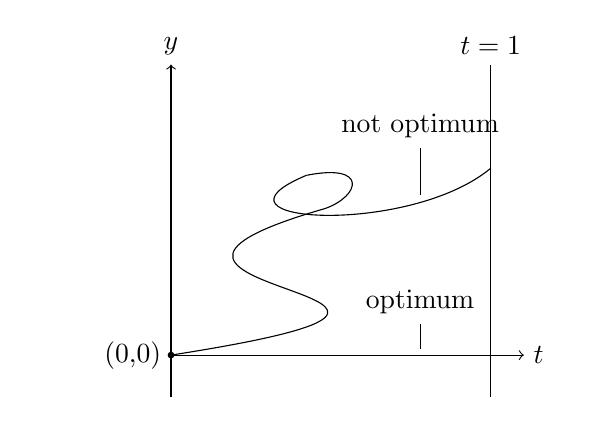
\begin{tikzpicture}[x=0.75pt,y=0.75pt,yscale=-1,xscale=1]
%uncomment if require: \path (0,319); %set diagram left start at 0, and has height of 319

%Curve Lines [id:da9395362233161386] 
\draw    (0,290) .. controls (196.2,259.4) and (-68.8,260.4) .. (74.2,219.4) ;
%Curve Lines [id:da4305029991293019] 
\draw    (65.2,203.4) .. controls (10.2,226.4) and (114.5,232.9) .. (154,200) ;
%Curve Lines [id:da9651462462408447] 
\draw    (65.2,203.4) .. controls (95.2,197.4) and (91.2,213.4) .. (74.2,219.4) ;
%Straight Lines [id:da18765309009648878] 
\draw[->]    (0,290) -- (170,290) node [right] {$t$} ;
\draw    (154,310) -- (154,150) node [above] {$t=1$} ;
\draw[->]    (0,310) -- (0,150) node [above] {$y$} ;
 
\filldraw [black]  (0,290) circle (1pt) node [left] {(0,0)}  ;

\draw (120,287) -- (120,275) node [above] {optimum} ; 
\draw (120,213) -- (120,190) node [above] {not optimum} ; 
\end{tikzpicture}
\caption{The shortest distance} %最终文档中希望显示的图片标题
\label{Fig11.1} %用于文内引用的标签
\end{figure}

Consider the path of minimum length between the points (0,0) and (1,0) in the plane; see Figure \ref{Fig11.1}. Call the horizontal coordinate $t$ and the vertical coordinate $y$. It is clear that any path which loops or winds cannot be of minimum length, because we can simply omit the loop or an S-shape to get a shorter one. We can therefore restrict discussion to the case where $y$ is a single-valued function of $t$. The distance between the adjacent points $(t,y)$ and $(t + dt,y + dy)$ is $[(dt)^2 + (dy)^2]^{1/2}$. Let $dy/dt = z$, the control variable. Then we are to maximize
\begin{equation} \label{equa11.23}
 - \int_0^1 [1+z(t)^2]^{1/2} dt
\end{equation}
subject to 
\begin{equation} \label{equa11.24}
  \dot{y}(t) = z(t)
\end{equation}
and $y(0)=y(1)=0$.

To use the Maximum Principle, define the Hamiltonian
\begin{equation} \label{equa11.25}
  H = -(1+z^2)^{1/2} + \pi z
\end{equation}
The first-order condition for $z$ to maximize this is
\begin{equation*}
  -(1+z^2)^{-1/2}z + \pi = 0
\end{equation*}
which simplifies to
\begin{equation} \label{equa11.26}
   z = \pi / (1-\pi^2)^{1/2}
\end{equation}
Then the maximized Hamiltonian is 
\begin{equation} \label{equa11.27}
  H^* = -(1-\pi^2)^{1/2}
\end{equation}

Now the two differential equations are
\begin{equation} \label{equa11.28}
  \dot{y} = \partial H^* / \partial \pi = \pi / (1-\pi^2)^{1/2}
\end{equation}
and
\begin{equation} \label{equa11.29}
  \dot{\pi} = - \partial H^* / \partial y = 0
\end{equation}
Thus $\pi$ is constant along the optimal path, and then so is $z$. But the only constant $z$ that will keep $y(1) = y(0)$ is zero. Thus the shortest path is the horizontal straight line joining (0,0) and (1,0).

We can apply Dynamic Programming and consider a somewhat more general problem, namely finding the shortest line joining (0,0) to the liner $t= 1$. First we consider the subproblem joining (0,0) to the general point $(T, y)$ with $T > 0$ but $y$ unconstrained. The theory above continues to apply, and we see that the straight line $y(t) = ty/ T $ does the job. Now it remains to choose $y$ optimally. The transversality condition for that is $\pi(T) = 0$. Since $\pi$ is constant along the optimal path, it must be zero everywhere. Then $z$ must be zero, and therefore $y(T) = 0$ is optimal. In other words, the shortest path from a point to a line is the straight line from the point and perpendicular to the given line.

\section*{Exercises}

\subsubsection*{\textit{Exercise 11.1: Search}}

Consider a variant of the search problem of Example 11.1. Suppose that the searcher can return to old jobs that he had rejected. So at any time, the state variable $x$ is the best offer he had observed up to that point. If he rejects this, searches and observes $y$, then next period he will start with the better of $x$ and $y$. Thus instead of (\ref{equa11.14}) we have
\begin{equation*}
  V_n(x) = \max \ \{ x(1-\delta^n)/(1-\delta), \ \delta E[V_{n-1}(\max (x,y)) ] \  \}
\end{equation*}
Show that there is a reservation wage $x_n^*$, and that the sequence of reservation wages is increasing in $n$. Write down the Bellman Equation as $n$ goes to infinity, and characterize its $x^*$. Note that
\begin{equation*}
\begin{array}{rl}
 E[V(\max(x,y))] = & \int_0^x V(x) \phi(y) dy + \int_x^\infty V(y) \phi(y) dy \\
                 = & V(x) \Phi(x) + \int_x^\infty V(y) \phi(y) dy 
\end{array}
\end{equation*}

\subsubsection*{\textit{Exercise 11.2: Intensity of Research Effort}}

The research and development needed for a new product consists of completion of a number of stages. Think of these as a continuum of length $L$. If $x(t)$ stages are completed at time $t$, and flow cost $c(t)$ is incurred on the R\&D program at this time, then the completion process evolves according to the differential equation
\begin{equation*}
  \dot{x} = f(x)
\end{equation*}
When all $L$ stages are completed, a reward $R$ accrues. If this occurs at time $T$, and $r>0$ is the rate of interest, the net present value of the program is 
\begin{equation*}
  R e^{-rT} - \int_0^T c(t) e^{-rt}dt
\end{equation*}
The aim is to choose the completion time $T$ and the profile of costs $c(t)$ over $[0,T]$ to maximize this.

Define $V(x)$ to be the value function for the corresponding problem that starts with $x$ stages completed. Applying Bellman's Principle over an initial small time interval $dt$, we have
\begin{equation*}
 V(x) = \mathop{\max}\limits_c \ \{ -cdt + V[x+ f(c)dt]e^{-rdt} \}
\end{equation*}
Expanding the right-hand side in a Taylor series as in the derivation of (\ref{equa11.5}), convert this into
\begin{equation} \label{equa11.30}
 r V(x) = \mathop{\max}\limits_c \ [ V^\prime(x)f(c) - c ]
\end{equation}

For the case $f(c) = c^\alpha$, with $0<\alpha <1$, the maximization in (\ref{equa11.30}) can be performed explicitly. Show that it yields
\begin{equation*}
   V^\prime(x) = \beta V(x)^{1-\alpha}
\end{equation*}
where $\beta$ is a known constant that depends on $r$ and $\alpha$. Solve this to show that
\begin{equation} \label{equa11.31}
  V(x)^\alpha = R^\alpha + \alpha \beta (x-L)
\end{equation}

Deduce that $V$ is a convex function, and therefore that the optimal intensity of research effort starts at a low level, and rises as more stages get completed. (Try offering this as an excuse for procrastination to your teachers, bosses etc.)

If $L$ is large enough, it may be optimal not to embark on this program of research at all. Find the limit on $L$. Solve the whole problem using the Maximum Principle.

How can the problem be modified to allow for uncertainty in the progress of research?








